%% ==============
\chapter{Evaluation}
\label{ch:Evaluation}
%% ==============
In this chapter we compare all the techniques we implemented with plain uniform and power-based Next Event Estimation and PBRTs implementation. We try to point out the strength and weaknesses of the techniques for certain kind of scenes and scenarios. In this context, we mainly argue about image quality, time and memory. We compare time and memory consumption based on the Root Mean Squared Error (RMSE) metric from equation~\ref{eq:rmse}. Where $Y_i$ is the vector of pixels of length $n$ of our reference image and $\widetilde{Y}_i$ is the vector of pixels of the compared image. Note that for unbiased techniques the variance $\sigma^2$ is equal to the MSE; hence we use both interchangeably in various contexts. 

\begin{align}\label{eq:mse}
\text{MSE} = \frac{1}{n}\sum_{i=1}^{n}\abs{Y_i - \widetilde{Y}_i}^2
\end{align}
\begin{align}\label{eq:rmse}
\text{RMSE} = \sqrt{\text{MSE}}
\end{align}


We often plot and compare based on RMSE; therefore the RMSE is an estimator for our image quality. When we argue about image quality we rather refer to the perceived image quality\footnote{The RMSE in itself has a perception component because of the square. The RMSE is a very commonly used estimator; nonetheless one could imagine using a metric which does reflect human perception more closely, see for example the structural similarity index (SSIM) \parencite{DBLP:journals/tip/WangBSS04}. This usually leads to problems with subjectivity.}, in our case this usually is determined by whether sensible artifacts are present. Figure~\ref{fig:intComparison} illustrates how the MSE and subjective image quality can differ. As all the compared techniques are unbiased, given unlimited time, all of them would converge to the same image. Artifacts are usually areas or edges which will converge very slowly, in practice maybe never. When we say a technique has a bad image quality, we mean that artifacts are present. 

As the standard deviation is proportional to the inverse root of the number of pixel samples (equation~\ref{eq:sigmaCor}) it quickly becomes unfeasible to converge an image by further increasing $N$. For this reason, increasing the efficiency per pixel sample is crucial.

\begin{align}\label{eq:sigmaCor}
\sigma \sim \frac{1}{\sqrt{N}}
\end{align}

We optimized our analysis to the 128 to 2048 samples per pixel range\unsure{correct? Whats the sweetspot?}, as this is a common range for real-world production. After an introduction into our setup and general test environment in the next section~\ref{sec:setup}, we continue into the most interesting part: equal time comparisons in section~\ref{sec:etc}.


\begin{figure}
\centering
\begin{subfigure}[b]{1\textwidth}
   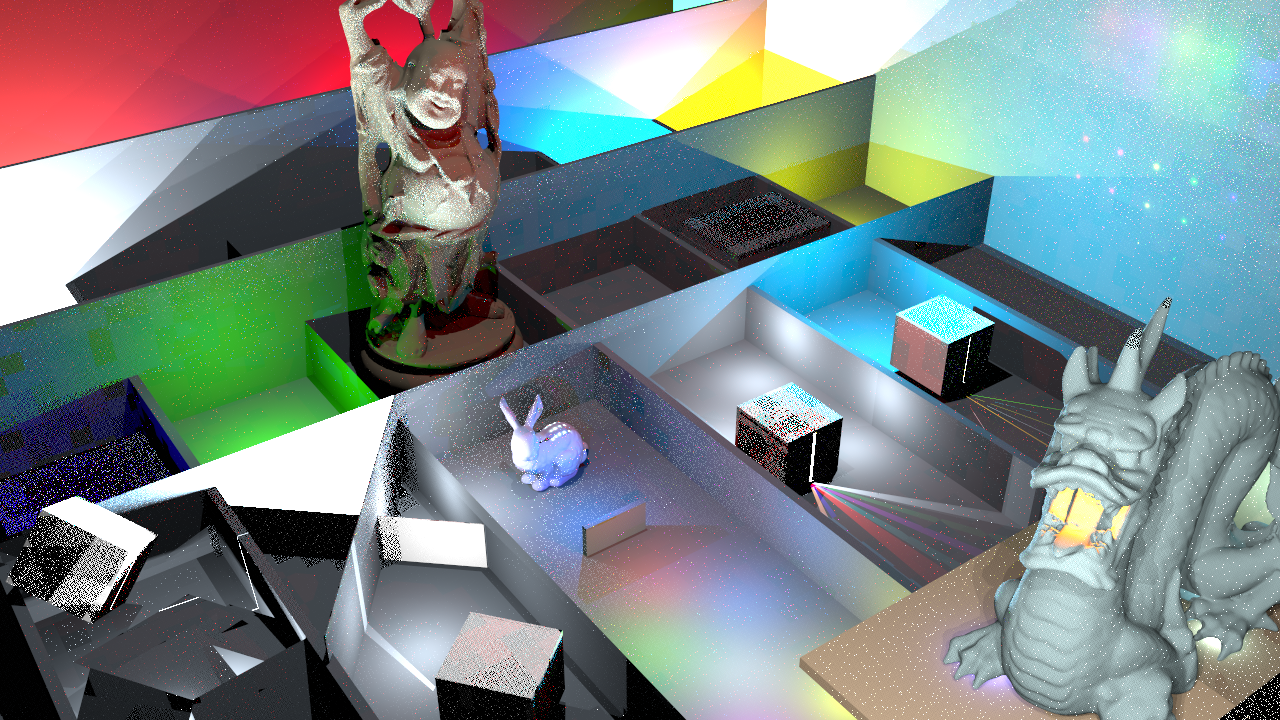
\includegraphics[width=1\linewidth]{figures/examples/StanfordMuseum_pvox_ps512_t503_icdf-0_pc96000k_mc0,1_Vox96_8854.png}
   \caption{Stanford-Museum rendered with 512 samples per pixel with \textit{Cdfgrid} and no interpolation.}
   \label{fig:SMnoInt} 
\end{subfigure}

\begin{subfigure}[b]{1\textwidth}
   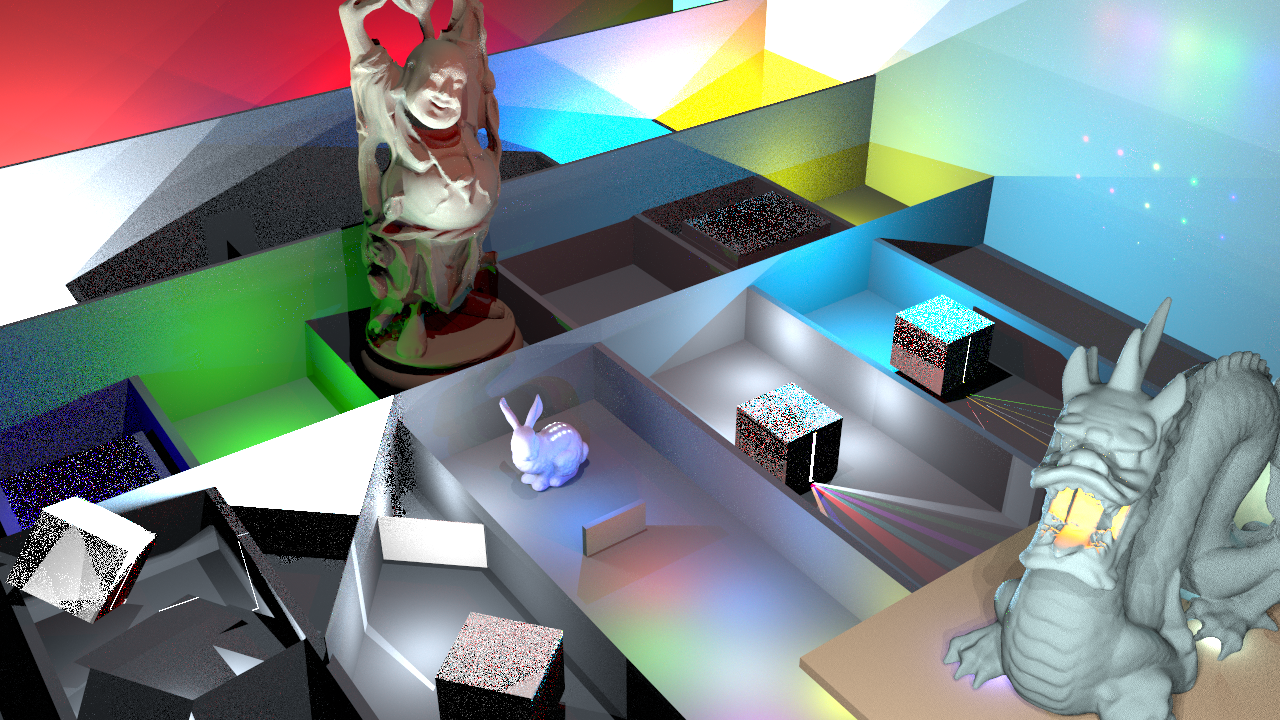
\includegraphics[width=1\linewidth]{figures/examples/StanfordMuseum_pvox_ps512_t723_icdf-1_pc128000k_mc0,1_Vox64_17574.png}
   \caption{Stanford-Museum rendered with 512 samples per pixel with \textit{Cdfgrid} and trilinear interpolation.}
   \label{fig:SMInt}
\end{subfigure}

\caption{A visual comparison of no interpolation versus trilinear interpolation. Even though we already have a rather high sample per pixel count, (a) shows many clear variance edges of the underlying grid cells and various artifacts across the scene. Also, it is remarkable how many fireflies are visible and how almost none of them are present in (b). It is quite apparent that a human observer would grade the image quality of (b) much higher, but surprisingly the RMSE of (a) is significantly smaller, $39.8$ versus $47.3$. The reason being, that aside of the fireflies and artifacts, the majority of pixels in (a) are less noisy. The difference in noise is less apparent at first, but is well illustrated on the white/gray wall to the left of the Buddha.}
\label{fig:intComparison}
\end{figure}


\section{Setup}
\label{sec:setup}
The test machine we use for comparisons is an Intel i7-4790K CPU @ 4GHz, 32 GB RAM, running on Windows 10 64-Bit. Images are produced by PBRT-v3, forked on March 30\footnote{Latest commit before the fork: \\ \url{https://github.com/mmp/pbrt-v3/commit/42c42c194bab970d8adc3f6b5e3afbbc172c3375}}. PNEE techniques are added on top of this fork; the complete implementation can be found at \url{https://github.com/AndiMiko/pbrt-v3}.

\subsection{Problem cases}

We tried to identify problematic light and object constellations, which are causing trouble for various kinds of techniques. The most prominent and comprehensible scenarios are to be covered below. 

\begin{description}
    \item[1. High Frequency.] Rapid changes to adjacent pixels can happen for two main reasons. Either there is a physical edge and thus the rays from the eye hit another object, or an object cast a hard shadow. The human observer is more forgiving when the variance changes together with the object material, while variance changes for the latter scenario usually are more irritating. With a lot fine shadows respectively strong light sources casting sharp light edges choosing the correct light source to sample can get tricky. A powerful light source can dominate an estimating data structure but may only be visible in a few spots. An estimator thus can quickly become bad while it was perfectly fine for a neighboring pixel. 
    \item[2. Level of Detail.] Highly varying object sizes and as such potential detail is the cause for a set of well-known problems in computer graphics. Especially, the choice of data structures is affected. A data structure can store a lot of data and thus spend a many resources on some big object but in the end the camera might only focus on a different tiny detail and as such make most of the data useless. This problems are usually addressed with adaptive data structures.
    \item[3. High variation of light power.] Some algorithms rely on a correlation between incident flux on a shading point and the power of a light source. This is the basis for the power-based technique compared to \textit{Uniform}. Also, the number of photons shot from a light source can be based on the light power and thus its alleged importance. This assumption is often useful, but can quickly cause problems when a strong light source is occluded close to a small light source which illuminates important details.
    \item[4. High number of contributing light sources.] The construction and lookup times of the acceleration data structures have to scale well, so that even in the case that a shading point is illuminated by many light sources rendering can stay efficient.
    \item[5. Non-axis aligned planes.] Skewed planes usually won't alight with the boundaries of the underlying data structures unless data structures like a BSP tree are used. Especially, rigid data structures like a grid can produce artifacts when the estimator seemingly arbitrarily changes. 
    \item[6. Highly occluded areas.] Large dark areas where most parts are occluded except a few spots where just a handful of photons may arrive can cause problems when trying to build meaningful estimators. Adaptive techniques may increase their search radius which can lead to unexpected behavior. Or estimators can't be build meaningfully with too few photons available.
    \item[7. Tiny but important solid angles.] The difference between a black box and an illuminated box can be a tiny hole or crack where a lot of light may enter and then scatter within. Also a small object that gets illuminated by a powerful but distant light source, e.g., the sun. The solid angle might be so tiny, that it is numerically very unlikely that photons would ever hit the object, but it may still be the main source of brightness.
\label{li:problemcases}
\end{description} 

\subsection{Test scenes}

We designed a special scene, called \textit{Stanford-Museum}, for most of the comparisons we present in this chapter. This scene covers all aforementioned problem cases and thus gives a good impression about strengths and weaknesses of each technique. The simplicity of the scene allows the reader to clearly correlate variance with the problem cases, but ultimately does not provide a photorealistic appeal. On the other hand, we present two more scenes, \textit{San Miguel} and \textit{Zero-day}, for a comparison on real scenes with all sorts of details.

\paragraph{Stanford-Museum}
\label{sec:stanfordmuseum}
\begin{figure}[ht]\centering
\captionsetup[subfigure]{labelformat=empty}

\begin{tikzpicture}[zoomboxarray, zoomboxes below, zoomboxarray inner gap=0.4cm,
zoomboxarray columns=4, zoomboxarray rows=2,remember picture, black and white]
   \node [image node] {
   \setcounter{zoombox}{0} 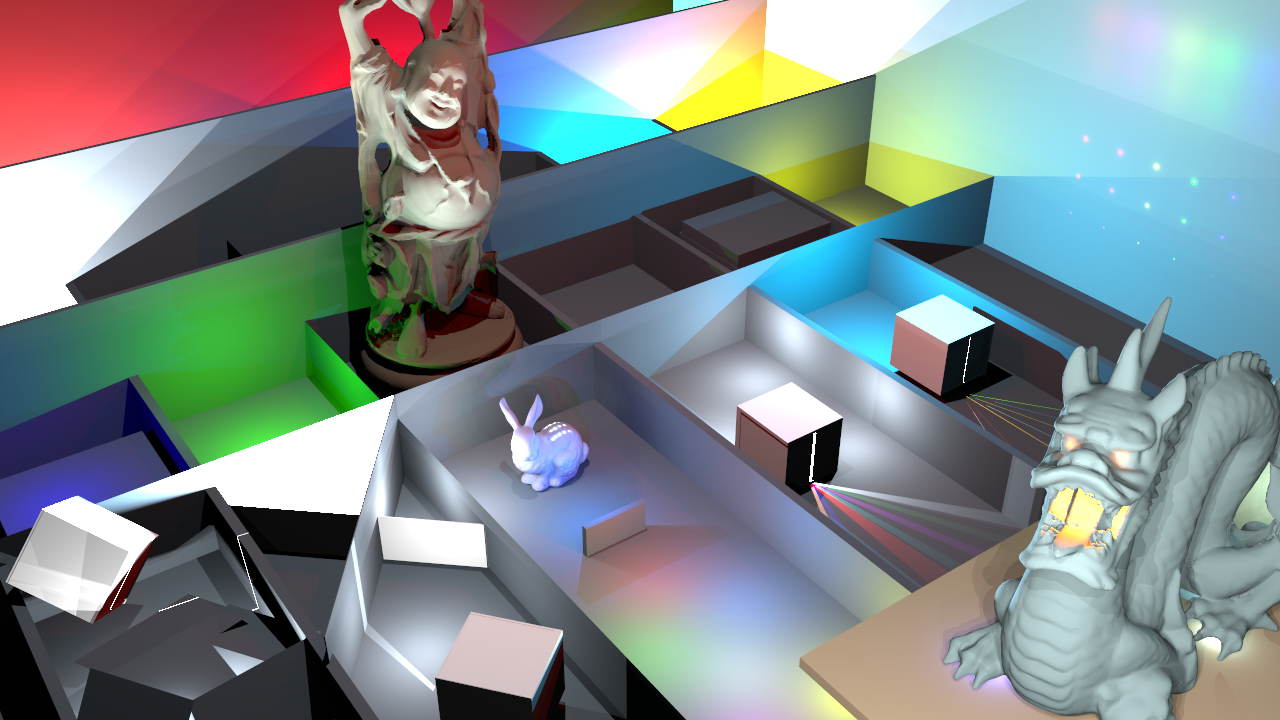
\includegraphics[width=1\textwidth]{figures/StanfordMuseum_ref.png}};
   
   \zoombox[magnification=0.8, color code=red]{0.85,0.3}
   \zoombox[magnification=1.5, color code=yellow]{0.334,0.78}
   
   \zoombox[magnification=2.3, color code=green]{0.767,0.47}
   \zoombox[magnification=1.4, color code=olive]{0.895,0.79}
   
   \zoombox[magnification=2, color code=brown]{0.285,0.32}
   \zoombox[magnification=1.3, color code=blue]{0.11,0.2}
   
   \zoombox[magnification=2, color code=cyan]{0.085,0.63}
   \zoombox[magnification=2, color code=pink]{0.6,0.68}

\end{tikzpicture}
\begin{tikzpicture}[overlay,remember picture]

\foreach \X in {1,...,\thezoombox}
   {\node[anchor=south,yshift=-13pt] at (zoombox-\X.south) 
   {\tiny (\X)};}
   \setcounter{zoombox}{0} 
\end{tikzpicture}

\caption{The reference image for \textit{Stanford-Museum} sampled with PBRTs directlighting integrator. Instead of NEE every light source is queried for any shading point. Max depth is one, thus no indirect illumination is present. All phenomenons from listing~\ref{li:problemcases} and more appear in this scene. Detailed descriptions and intentions of the zoomed areas are listed in~\ref{li:stanfordmuseum}.
}
\label{fig:stanfordmuseumref}
\end{figure}

We describe the most important problem cases we had in mind when designing the Stanford-Museum scene in figure~\ref{fig:stanfordmuseumref}, which is the reference image we calculate the RMSE against. The scene contains 4058 light sources, all of whom are point light sources. We chose point light sources because sampling a point on an area light source is not a concern of PNEE, thus reducing variance from other effects does disclose artifacts produced by our techniques more clearly. We also render the scene with a path tracer with a max depth parameter of one, again, using the same argument, as depth introduces variance from the indirect lighting term of the path tracer. Additionally, this makes rendering a nearly perfect reference image possible, by using PBRTs direct lighting integrator, which samples all point light sources for every intersection point. The reference image is rendered with 128 samples per pixel in 17 hours on our test machine and aside from anti-aliasing should be close to perfect. 

\begin{itemize}
    \item[(1)] The dragon is 20 times smaller than the Buddha but is very close to the camera and as such takes up almost the same screen space. Several low-intensity point lights illuminate the dragon. The difference in size, as well as light intensity, constitute typical problem cases with LOD. Especially the illumination of the eyes is a rather extreme case, light source intensity is roughly 200.000 times less compared to the strongest light sources in the scene. Additionally, the left outline of the dragon is illuminated by various light sources from bellow in the scene, where the dragon takes up only an incredibly small solid angle and thus photons are very unlikely to hit the dragon.
    \item[(2)] The Buddha stands out of all cells and as such is illuminated by almost all visible light sources in this scene. This is particularly a problem for example with \textit{Photontree}. There might be more light sources influencing a shading point, than the total number of nearest neighbors we collect. High geometric detail and blending of many light colors make the Buddha prone to fireflies.  All three Stanford models are also intended to add complexity for intersection tests to various parts of the scene. 
    \item[(3)] The box has a very tiny split from which it casts long range, very bright, very thin and high frequent light rays. Additionally, many photons are stuck within the thin-walled box, which highly complicates building good estimators with PNEE on the outside. Several more of this boxes with varying properties and surroundings are present in the scene. 
    \item[(4)] Similar to the Buddha this plane wall is illuminated by many light sources in the scene. Additionally, there is a matrix of point lights with varying brightness, distance, and color. This variety has to be mapped to smooth transitions and high frequencies accordingly. Similar scenarios to this one do also appear in other parts of the scene, for example in front of the bunny, also with many smooth transitions, but where difficulties brought by global illumination are replaced with many local soft shadows. 
    \item[(5)] A cluster of roughly 1000 light sources. Only thin, non-axis-aligned walls separate it from several distinct lightning scenarios. Very high exposure (unintentionally) breaks anti-aliasing. Most light sources influence the Buddha softly from below. 
    \item[(6)] Several non-axis-aligned thin walls cover up a small cluster of light sources and cast thin, high frequent light rays in many directions. Especially the rays casted onto the skewed box, where photons from within the box, as mentioned in (3), do no good for our estimators, do constitute a tricky shading scenario in various manners.
    \item[(7)] Several strong light sources cast long range, smoothly fading, but sharp-edged light rays. A similar scenario is present on the other side of the Buddha, where colors also blend together. The rays closely pass quite dark cells. Again, strong light sources behind a thin wall interfere with our photon collection algorithms.
    \item[(8)] A completely occluded light cluster with roughly 1000 light sources. In a real scene, this might be a different room of a house for example. There are four such occluded clusters in the scene.
\label{li:stanfordmuseum}
\end{itemize}
\paragraph{San Miguel}
\label{sec:sanmiguel}
San Miguel by \textcite{Sanmiguel} is a popular scene and was on the book cover of the second edition of PBRT. It offers a highly detailed and photorealistic appeal and therefore is great for illustrative purposes and evaluating our techniques in a high detail scene. As such it also serves as a realistic stress test which includes all kinds of materials, reflections, transparencies, and shapes. Many of which were intentionally spared in the design of \textit{Stanford-Museum}. We intended San Miguel to be a realistic test to make sure everything works as intended. The original scene only has one light source, a distant environment light, which indeed was the only cause for problems for PNEE. Due to the current implementation, which very well may get improved in the future, the photon count had to be set higher than it normally should have. This was the only found issue.

The scene had to be enriched with more light sources to function as a test scene for our purpose. As the original c4d files are not available anymore the light sources had to be pasted manually.\unsure{ist das unwichtig? rauslassen?} There are several closed rooms in all directions to the yard. All rooms got augmented with clusters of light sources, which may constitute some realistic illumination within the rooms, but do not affect the yard respectively the view of the rendered image. In total there are 1274 light sources in the scene, of which only 13 do actually affect the viewport. This was needed to be able to render a meaningful reference image. Therefore, all light sources were removed, except the 13 significant ones, and then the scene was rendered with PBRTs spatial technique with 8192 samples per pixel in 16.5 hours.\footnote{This might give spatial a slight advantage in later MSE calculations due to the general alignment of potential variance edges. This effect should be minimal though. Creating a fully unbiased reference was not feasible.} This yielded a good reference image, while all other images are rendered with all 1274 light sources, even though we know they should actually not affect the desired image.

\paragraph{Zero-Day}

Zero-Day by \textcite{Beeple} is also a fascinating scene that actually provides many light sources natively. With 8916 light sources it has by far the most light sources in our tests, but interestingly still doesn't make the strongest argument for PNEE. Almost all light sources are very weak and the scene is quite open, thus occlusion does not play a significant role; therefore the weaknesses of PBRTs spatial are not revealed.

The reference image was rendered with \textit{Spatial} due to the lack of a better option. With 12288 ps, the Sobol sampler, a max depth of seven and a 960x420 resolution the rendering took a bit over 12 hours. The image still shows a few fireflies and comparison against \textit{Spatial} itself is obviously biased. We used the Sobol sampler but for the comparison use the Halton sampler to reduce the correlation, so that the same random samples won't create the exact same fireflies at least.



\FloatBarrier
\subsection{Techniques}

We give a brief overview of the techniques that we identified as interesting for comparison. \textit{Uniform} and \textit{Power} sampling are naive techniques that are natively implemented in PBRT. Additionally, PBRTs just recently released take on many light sampling is referred to as \textit{Spatial}, see chapter~\ref{ch:Prev}. We compare these three existing techniques with our own techniques \textit{Cdfgrid}, \textit{Photontree} and \textit{Cdftree} introduced in Table~\ref{tb:techniques}. All three of our techniques use interpolation, as this produces the cleanest results for human observers. Nonetheless, we also list \textit{Cdfgrid no int}, which uses no interpolation. The images produced by this technique usually contain artifacts, but nonetheless performs very well on the MSE plots as the overall variance is better. For later plots, we spare previously clearly worse performing techniques to focus our discussion.

\subsection{Parameter Comparison}

\unsure{remove this section? Too much dump data, not highly interesting unless someone wants to reimplement}

%%%%%%%%%%%%%%%%%
\label{ch:ev:photontree}

%%%%%%%%%%%%%%%%%
\label{ch:ev:cdftree}

%%%%%%%%%%%%%%%%%%%%

\label{ch:ev:photonsampling}


%%%%%%%%%%%%%%%%%%%%%%%
\label{ch:ev:uniformfloor}

% which parameters did we try to configure. Which parameters turned out to be good and will be set as fixed?

\section{Equal time comparisons}
\label{sec:etc}
In this section, we compare and discuss our results for various techniques. We show two kinds of graphs: a $\sigma$ versus time in seconds graph and a $\sigma$ versus number of pixel samples (ps) graph; all in logarithmic scales. The time-plots make sense intuitively. The ps-plots are interesting because our test scenes, for the most part, do not contain fancy techniques or features that significantly increase rendering times per pixel (as e.g. \textit{Photontree} does). In real-world renderers though these techniques may very well exist and as such the proportional increase of rendering time per pixel sample introduced by PNEE might be significantly lowered; which in turn would make the ps-plot more significant. Additionally, it may be a better indication of how efficient a technique is disregarding the potentially sub-optimal implementation.

All data for the results showed and discussed here are available at \url{https://github.com/AndiMiko/PNEE-data}. The data contains the source for the graphs, calculated MSE and RMSE, all result images in .exr format and equally named .txt files which contain a copy of the original .pbrt configuration file and some additional rendering run logs \& analytics.

\subsection{Stanford-Museum}

\begin{figure}
    \centering
    \begin{subfigure}{.5\textwidth}
      \centering
        \adjincludegraphics[width=1\textwidth, trim={{.06\width} {.08\height} {.371\width} {.15\height}},clip]{figures/plots/SM_Main_t.pdf}
        \caption{}
        \label{fig:smmain_t}
    \end{subfigure}%
    \begin{subfigure}{.5\textwidth}
        \adjincludegraphics[width=1\textwidth, trim={{.06\width} {.08\height} {.371\width} {.15\height}},clip]{figures/plots/SM_Main_ps.pdf}
        \caption{}
        \label{fig:smmain_ps}
    \end{subfigure}
    \caption{Stanford-Museum time-$\sigma$ and ps-$\sigma$ log-log plots.}
    \label{fig:smmain}
\end{figure}


Considering that the plots in figure~\ref{fig:smmain} are logarithmic on both scales we see vast differences between the techniques; we discuss the most interesting phenomena here. Table~\ref{tb:sm_settings} shows the used settings. The time-plot~\ref{fig:smmain_t} includes the preprocessing time. For this reason, PNEE techniques start at a later point, usually around 100 seconds. Settings may be adjusted for specifically desired rendering times, e.g. to better compete in the sub 100 second range; in our case, we decided to have the same render settings for all pixel sample times, as we mainly aim for the most interesting comparisons in the middle section of the plots. Log-log plots should usually be a straight line---we explain the observable curvature in~\ref{fig:smmain_t} with the preprocessing time. The graph is quickly catching up what it has lost due to the preprocess. The ps-plot~\ref{fig:smmain_ps} confirms this: as preprocessing time doesn't play a role the curvature in the beginning is gone. In the end, we see the opposite effect. As the image is already very well converged the very last errors are probably not very well estimated by PNEE anymore. For this reason, the PNEE techniques seem to slowly loose the very large advantage they previously had and gradually converge against what is only solvable with brute force. Slight imperfections in the reference image may also be the cause to this.\footnote{We have the comfort of being able to assume to have a nearly perfect reference image in a rather complex scene, as discussed in~\ref{sec:stanfordmuseum}. For the other scenes we do not have this possibility and for this reason, we are not even considering this high number of samples per pixels in the upcoming plots.} We also speculate that it might be possible to straighten the PNEE plots by proportionally scale the preprocessing complexity with the desired pixel samples. The advantage should therefore not fall off at later stages. Anyhow, note, that the illustrated pixel sample numbers are already far above usual and the plots are still very far away from actually converging together. The curvature begins slightly at around 1024 samples per pixel, while data at above 4096 samples per pixel is mostly only interesting for scientific purposes. This is also reflected by the anomalies at around 16K pixel samples. Surprisingly, PNEE techniques are not affected, whereas \textit{Uniform}, \textit{Power} and \textit{Spatial} are. While we are not certain, our explanation is that the Halton sampler used by PBRT ran out of random numbers and starts looping there. We found slight correlative variance edges/lines that indicated this, especially in the completely broken out \textit{Uniform} 32K ps image.

Focusing on the actual graphs we see a very clear winner: \textit{Cdfgrid (no int)}. The naive version performs slightly better than its interpolated counterpart. The ps-plot reveals that this advantage is mostly due to the additional processing cost of the interpolation, as graphs are almost glued together there. Variance edges are nicely smoothed but overall variance increases. What weights stronger should likely be scene dependent. Even though by the numbers \textit{Cdfgrid no int} may be regarded as best performing in presented plots we are confident that a human observer would choose \textit{Cdfgrid} as the clear winner, refer to figure~\ref{fig:intComparison}.

The \textit{Spatial} graph moves very inconsistently and interestingly, at first glance, the slope in the middle area might suggest that it should surpass all techniques at a later stage. A more in-depth analysis reveals that the inverted effect that we previously discussed about the curvature appears to be responsible. The technique creates several strong artifacts which give it a negative headstart, while it is correcting its own mistakes the slope is heavily favored. Mentally connecting the 16 ps and 8K ps dots in the ps- and time-plot might give a good indication of how efficient the technique would be if it would actually work in these scenarios (good but still worse than PNEE). The very same effect appears to cause the bump in the 64 ps point of the \textit{Cdftree} technique. This highlights problems with the consistency of both techniques, nonetheless, these problems may rarely appear in naturally modeled scenes, as such the theoretical performance can be regarded as quite good, with both techniques occupying the midfield. 

As expected, \textit{Uniform} and \textit{Power} are performing significantly worse. The only arguments going for them are that they have no settings and the rendered images have a very even \enquote{undone-look}, as there are no artifacts or any differences in variance by design. Other than that they are clearly not suited for such scenes, even tough with roughly a thousand light sources we are far away from imaginable extremes.

\textit{Photontree} was a surprise on the other hand. While early tests already indicated that the workload within the integrator is clearly too high the final results on the time-graph are quite striking. We want to further highlight the ps-graph. While results look much better there it is still highly surprising that it merely competes with the naive techniques. We expected clearly better results on the ps-graph, but apparently, there are too many artifacts as seen in figure~\ref{fig:discontinuityEdges}\footnote{The artifacts are much more subtle in the end results.}. Visually comparing the 4K ps image of \textit{Photontree} and \textit{Uniform} was even more irritating\todo{add figure to appendix?}. We had to double-check whether the MSE calculation was done properly, since the \textit{Photontree} image looked so much better except for a few unpleasant artifacts. Indeed it appears that the square in the MSE calculation really kicks in here, the artifacts are heavily punished in our plots. In conclusion, on the ps-plot we would easily favor the \textit{Photontree} images, but the time-plot clearly deprives \textit{Photontree} of any viability.

Overall the log-log plots are already indicating the vast differences, but visually comparing even more so highlights the gaps. The results range from completely unusable to excellent\todo{add figure of all techniques?}. Comparing, for example, the 128 ps \textit{Cdfgrid} image rendered in 159 seconds with the 16K ps \textit{Uniform} image rendered in 14551 seconds and similar MSE the speedup lies at roughly 90x. \textit{Cdfgrid} does not only dominate the plots, but also its ease of use and visual comparison satisfy all demands.

\begin{center}

\begin{tabular*}{\textwidth}{@{}l @{\extracolsep{\fill}} llll@{}}\toprule
 & Cdfgrid no int & Cdfgrid & Cdftree & Photontree~~~ \\ \midrule

Photon count & 96 mil & 96 mil & 50 mil & 96 mil\\
Cdf count & --- & --- & 150.000 & --- \\
Max grid cells & 96 & 96 & --- & ---  \\
Uniform floor & 0.1 & 0.1 & 0.1 & 0.1  \\
Collection Method & --- & --- & NN & NN \\
Interpolation & none & trilinear & AKR & AKR \\
NN-count & --- & --- & 16 & 192 \\
Photon threshold & --- & --- & 20 & --- \\

\bottomrule
\end{tabular*}
\captionof{table}{Render settings for Stanford-Museum for the plots in figure~\ref{fig:smmain}.}
\label{tb:sm_settings}
\end{center}






\FloatBarrier
\subsection{San Miguel}

\begin{figure}
    \centering
    \begin{subfigure}{.5\textwidth}
      \centering
        \adjincludegraphics[width=1\textwidth, trim={{.06\width} {.08\height} {.371\width} {.15\height}},clip]{figures/plots/SanMiguel_main_t.pdf}
        \caption{}
        \label{fig:sanmain_t}
    \end{subfigure}%
    \begin{subfigure}{.5\textwidth}
        \adjincludegraphics[width=1\textwidth, trim={{.06\width} {.08\height} {.371\width} {.15\height}},clip]{figures/plots/SanMiguel_main_ps.pdf}
        \caption{}
        \label{fig:sanmain_ps}
    \end{subfigure}
    \caption{San Miguel time-$\sigma$ and ps-$\sigma$ log-log plots.}
    \label{fig:sanmain}
\end{figure}

Going into the San Miguel analysis we spared \textit{Photontree} because of its bad results and \textit{Cdfgrid no int} because results are very similar and all valuable insights were already made in the Stanford-Museum analysis. Checking the plots in figure~\ref{fig:sanmain} we again see the previously discussed phenomena like the curved graphs of the PNEE techniques. \textit{Spatial} is very straight now, as there is no specific scenario present that creates artifacts. Overall the plots look cleaner due to the absence of the high variety of problem cases as in Stanford-Museum. \textit{Uniform} and \textit{Power} swapped their ranking with a quite considerable gap. \textit{Power} and \textit{Cdfgrid} wiggle slightly for an unknown reason, but the effect is small enough to be potentially caused by randomness\unsure{Is this true? I don't have a better explanation. Better not to mention or what to say? Better word than randomness?} or potentially the bias of the reference image. \textit{Cdftree} is the only one appearing unstable, a visual comparison reveals one problematic area. It is very well possible that tuning the settings just a bit might already solve this issues, as this completely changes the dynamic of the underlying data structure---unfortunately in an unpredictable manner. Other than that results are really good and results even briefly surpass \textit{Cdfgrid} in the ps-graph. 

Nonetheless, overall \textit{Cdfgrid} does dominate this comparison as well. Visual comparison in figure~\ref{fig:migcomp} reflects what the graphs already have revealed. The high deviation of results compared to the Stanford-Museum plots illustrates that the efficiency of certain techniques is scene dependent. Used parameters are quite similar to Table~\ref{tb:sm_settings} and won't be listed again for this reason, but can be found in the Github repository.

\begin{figure}
    \centering
    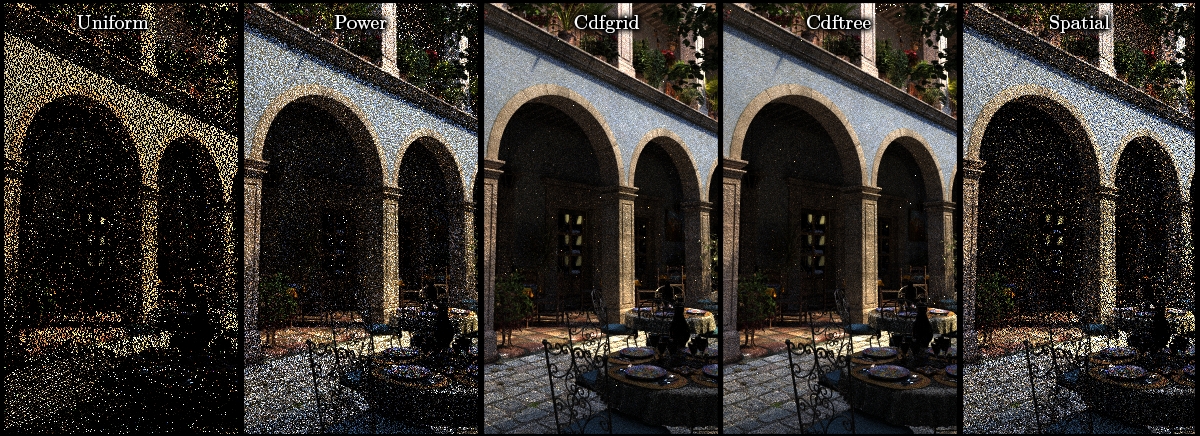
\includegraphics[width=1\textwidth]{figures/comparisons/Mig_comp_same_slimmer.png}
    \caption{Cropped San Miguel comparison of the 256 ps images.}
    \label{fig:migcomp}
\end{figure}
\unsure{which comparison image of San Miguel do you like more? Equal or whole image}

\FloatBarrier
\subsection{Zero-Day}

\begin{figure}
    \centering
    \begin{subfigure}{.5\textwidth}
      \centering
        \adjincludegraphics[width=1\textwidth, trim={{.06\width} {.08\height} {.371\width} {.15\height}},clip]{figures/plots/ZeroDay_main_t.pdf}
        \caption{}
        \label{fig:zd_t}
    \end{subfigure}%
    \begin{subfigure}{.5\textwidth}
        \adjincludegraphics[width=1\textwidth, trim={{.06\width} {.08\height} {.371\width} {.15\height}},clip]{figures/plots/ZeroDay_main_ps.pdf}
        \caption{}
        \label{fig:zd_ps}
    \end{subfigure}
    \caption{Zero-Day time-$\sigma$ and ps-$\sigma$ log-log plots.}
    \label{fig:zd}
\end{figure}

Zero-Day comparison graphs (figure~\ref{fig:zd}) are, unlike the first two. Having the most light sources of all test scenes reflects in the fact that \textit{Uniform} is performing even worse than before. Not even the 1024 ps image is remotely usable. On the other hand, it is remarkable how close \textit{Power}, \textit{Spatial} and \textit{Cdfgrid} compare. \textit{Power} performs well because most important contributions come from 2-3 important bigger light sources. Most other light sources are very weak yellow buttons, which are mainly sampled through rays directly hitting the area light instead of NEE.

The scene barely relies on occlusion. This shows that PNEEs unique advantage that it had in previous test scenes is gone. In that sense \textit{Spatial} essentially serves as a lower efficiency bound for PNEE. Without occlusion both techniques are practically equal. Note that the reference image is rendered with \textit{Spatial} itself, hence the comparison is even biased towards \textit{Spatial}. Nonetheless, \textit{Cdfgrid} has a slight edge even though interpolation was active. 

A visual comparison, once again is quite surprising. In fact, the MSE does not reflect the perceived noise; figure~\ref{fig:zdcomp} clearly shows that \textit{Power} has more noise pretty much everywhere, compared to relatively clean \textit{Cdfgrid} and \textit{Spatial}. We tried looking carefully for artifacts that could justify the similarity in MSE, but it remains a mystery.

\textit{Cdfgrid} and \textit{Spatial} perform basically equal both visually as well as in MSE. With a clear visual advantage they are both very likely to be preferred against \textit{Power}.


\todo{HALTON/SOBOL spatial}

\begin{figure}
    \centering
    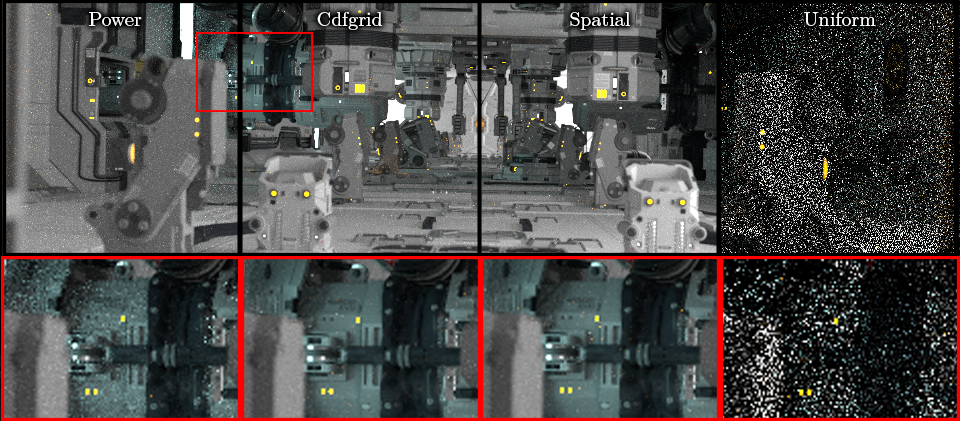
\includegraphics[width=1\textwidth]{figures/comparisons/ZDcomp_slim.png}
    \caption{Zero-Day comparison of the 512 ps images with increased exposure. }
    \label{fig:zdcomp}
\end{figure}


\FloatBarrier
\section{Memory comparison}

We initially expected \textit{Cdfgrid} to be memory-bound and as such the tradeoff between memory and time would become a key decision factor when choosing a rigid versus an adaptive data structure. As it turns out the memory consumption was not critical at all, with usage ranging between 1-5 GB for all techniques. We expected that with \textit{Cdfgrid} detail could be increased until it would be bound by memory, but in fact, image quality started dropping long before those boundaries were reached. This is due to the fact that cells get smaller throughout the whole scene and start destabilizing the technique. Too many small cells leave much more room for outliers which receive too few photons, or are placed in a very unfortunate position. While interpolation mitigates these problems for reasonably (still small) sized cells, at a certain degree artifacts start to sprout. The technique still works well but variance starts to increase with too much memory. \textit{Cdftree} has similar problems even amplified.  Additionally, as the evaluation in section~\ref{sec:etc} has shown \textit{Cdfgrid} was able to dominate without even needing to push memory boundaries. Other techniques proved to be less consistent in image quality and speed and as such memory hasn't become the decisive factor. 

\begin{center}
\begin{tabular*}{\textwidth}{@{}l @{\extracolsep{\fill}} llll@{}}\toprule
Uniform/Power & Spatial & Cdfgrid & Cdftree & Photontree~~~ \\ \midrule
0.14 GB & 0.23 GB\footnotemark[6] & 2.28 GB & 4.25 GB\footnotemark[7] & 4.8 GB\footnotemark[7]  \\
\bottomrule
\end{tabular*}
\captionof{table}{Total peak memory consumption during rendering Stanford-Museum with settings as in Table~\ref{tb:sm_settings}.}
\label{tb:memory}
\end{center}

\footnotetext[6]{Constantly growing. Apparently leaking memory.}
\footnotetext[7]{Roughly half of the memory is freed after the preprocess. A better implementation might be able to swap the memory if memory would have been an issue.}

In fact table~\ref{tb:memory} illustrates that memory consumption is dominated by the form of storage and not the data structure unlike our initial expectation. Photons already take up most of the space and with an increasing number of light sources (potentially millions) the photon count will linearly scale. On the other hand a grid does not have to be adjusted to the number of lights and while the complexity of each contained CDF grows, the practical memory consumption scales sub-linearly due to the utilization of sparse CDFs.

\section{Conclusion}

During this chapter, the advantage of utilizing an occlusion-aware technique like PNEE was clearly illustrated. \textit{Photontree} was ought to be the precision favorite but performance was unacceptable and surprisingly not even the ps-graph was convincing. \textit{Cdftree} has shown very promising rudiments but is hard to control and predict. The technique can certainly be further optimized notably on the clustering algorithm and adaptive parametrization. In general, parametrization was not as susceptible as we initially thought. After some induction, all techniques were used comfortably. Only the appearance of artifacts was kind of unpredictable and hurt the stability and otherwise excellent results of \textit{Cdftree} the most. 

Potentially due to the choice of test scenes \textit{Cdftree} was not able to utilize its biggest strength: Handling highly varying LOD. We designed the dragon in Stanford Museum for this reason, but apparently, it was not influential enough to let \textit{Cdfgrid} stand out. It is questionable how far LOD has to be stretched until it becomes a decisive factor. At that point in practice a designer probably would be comfortably removing large parts of the scene manually. Nevertheless, \textit{Cdftree}s performance on average scenes was still strong and persuasive and was only overshadowed by the performance of \textit{Cdfgrid}.

\textit{Cdfgrid} has shown to be stable, easy to operate and distinctively fast. The visual weaknesses of \textit{Cdfgrid no int} are remarkably well solved by trilinear interpolation with minimal cost. Suspected weaknesses on the memory consumption and LOD didn't turn out to be an issue. With hardly any drawbacks and constant top performance \textit{Cdfgrid} exceeded our expectations and appears to be a great choice for any lighting situation.
